\chapter{Simspark}
\label{cha:simspark}

In this section you find information about the messages that are sent from the
server to the agent (perceptors) and vice versa (effectors). A description of
the perceptors and effectors can also be found in \cite{SchillingJ} (German), \cite{Lekavy} (Slovak), and to some part in \cite{Vorst06} (concerns the older "spheres" simulation though, so some information is outdated).





%-SECTION-----------------------------------------------------------
%--------------------- General message format ----------------------
%-------------------------------------------------------------------
\section{General message format}
\label{sec:msgformat}
Messages from and to the server use S-expressions (short for symbolic
expressions) as their basic data structure. The basic idea of
S-expressions is very simple: they are either strings, or lists of
simpler S-expressions.  They are probably best known for their use in
the Lisp family of programming languages where they are used for both
code and data.

An advantage of using S-expressions over other data formats is that it
provides an easy to parse and compact syntax that is to some extent
still readable by humans for debug purposes. It is further easy to add
new sensors to the messages as the parser on the client side can
easily ignore unknown parts.

Messages exchanged between client and server use the default ASCII
character set, i.e. one character is encoded in a single byte. Further
each individual message is prefixed with the length of the payload
message. The length prefix is a 32 bit unsigned integer in network
order, i.e. big endian notation with the most significant bits
transferred first.





%-SECTION-----------------------------------------------------------
%--------------------------- Perceptors ----------------------------
%-------------------------------------------------------------------
\section{Perceptors}
\label{sec:perceptors}
Perceptors are used to sense the environment of the agent. They are sent from
the server to each agent and contain agent specific and perceptor specific
information about the environment and the agent itself. There are perceptors
that are available to all kinds of simulations and soccer specific perceptors.

% Klaus:do we have noise in perceptors?
% Joschka: only in some so far (e.g. vision); the joint perceptors, gyro, and touch perceptors don't have noise yet (should be on the ToDo list)





%-SUB-SECTION-------------------------------------------------------
%----------------------- General Perceptors ------------------------
%-------------------------------------------------------------------
\subsection{General Perceptors}
\label{sec:generalperceptors}
The perceptors described in this subsection are available to all types of
simulation. In other words they are not specific to the soccer environment.



%-SUB-SUB-SECTION---------------------------------------------------
%---------------------- HingeJoint Perceptor -----------------------
%-------------------------------------------------------------------
\subsubsection{HingeJoint Perceptor}
\label{sec:HJP}
A \emph{hinge joint perceptor} receives information about the angle of the
corresponding single axis hinge joint. It contains the identifier
``\texttt{HJ}'', the name of the specific perceptor (see robot
descriptions~\ref{cha:robots}) and the position angle of the axis in degrees.
Zero degrees corresponds to straightly aligned bodies. The position angle of
each hinge joint perceptor is sent every cycle. A hinge joint is displayed in
figure \ref{ode:hingejoint}.

\begin{figure}[htbp]
  \begin{center}
	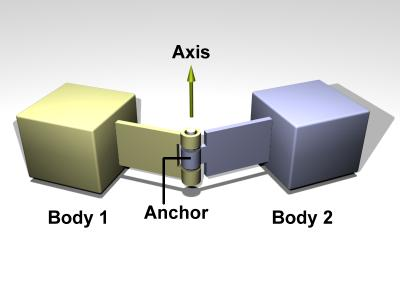
\includegraphics[scale=0.6]{fig/HingeJoint.png}
    \caption{Hinge Joint (\cite{ODEManual})}
    \label{ode:hingejoint}
  \end{center}
\end{figure}

%klaus: What is the zero degree position, is the above correct?
%Joschka: I don't think this is necessarily correct; to my knowledge, the zero position is determined by the orientation and position of the bodies at the time the joint is attached. Is this right?

\begin{itemize}
	\item[Message format:] \texttt{(HJ (n <name>) (ax <ax>))}
		\begin{itemize}
		  \item[\texttt{<name>} -] the name of the corresponding hinge joint
		  \item[\texttt{<ax>} -] the current position angle in degrees and an accuracy
		  of two digits
		\end{itemize}
	\item[Example message:] \texttt{(HJ (n laj3) (ax -1.02))}
	\item[Noise model:] None
\end{itemize}



%-SUB-SUB-SECTION---------------------------------------------------
%-------------------- UniversalJoint Perceptor ---------------------
%-------------------------------------------------------------------
\subsubsection{UniversalJoint Perceptor}
\label{sec:UJP}
A \emph{universal joint perceptor} receives information about the two angles of
the corresponding two axis universal joint. It contains the identifier
``\texttt{UJ}'', the name of the specific perceptor (see robot
descriptions~\ref{cha:robots}) and the position angles of the two axes in
degrees. Zero degrees corresponds to straightly aligned bodies. Like the hinge
joint, this perceptor is also a every-cycle-perceptor. A universal joint is
displayed in figure \ref{ode:universaljoint}.

\begin{figure}[htbp]
  \begin{center}
	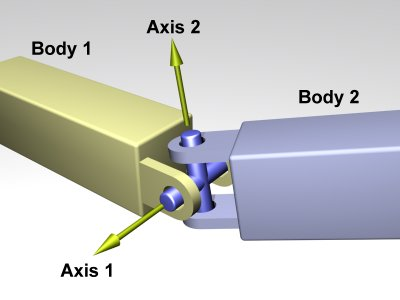
\includegraphics[scale=0.6]{fig/UniversalJoint.png}
    \caption{Universal Joint (\cite{ODEManual})}
    \label{ode:universaljoint}
  \end{center}
\end{figure}
 
\begin{itemize}
	\item[Message format:] \texttt{(UJ (n <name>) (ax1 <ax1>) (ax2 <ax2>))}
		\begin{itemize}
		  \item[\texttt{<name>} -] the name of the corresponding universal joint
		  \item[\texttt{<ax1> <ax2>} -] the current position angles of the two axes in
		  degrees and an accuracy of two digits
		\end{itemize}
	\item[Example message:] \texttt{(UJ (n laj1\_2) (ax1 -1.32) (ax2 2.00))}
	\item[Noise model:] None
\end{itemize}



%-SUB-SUB-SECTION---------------------------------------------------
%----------------------- GyroRate Perceptor ------------------------
%-------------------------------------------------------------------
\subsubsection{GyroRate Perceptor}
\label{sec:GYR}
The \emph{gyro rate perceptor} delivers information about the change in
orientation of a body with respect to the global coordinate system. The message
contains the ``\texttt{GYR}'' identifier, the name of the body to which the gyro
perceptor belongs and three rotation angles. These rotation angles describe the
change rates in orientation of the body during the last cycle. In other words
the current angular velocities along the three axes of freedom in degrees per
second ($deg/s$). To keep track of the orientation of the body, the information
to each gyro rate perceptor is sent every cycle.
% Note: The values given by this perceptor are related to the coordinate system of
% the body containing the perceptor.
\begin{itemize}
	\item[Message format:] \texttt{(GYR (n <name>) (rt <x> <y> <z>))}
		\begin{itemize}
		  \item[\texttt{<name>} -] the name of the body containing the
		  gyro rate perceptor (see robot descriptions \ref{cha:robots})
		  \item[\texttt{<x> <y> <z>} -] the current angular velocities along the
		  three axes of freedom of the parent body in $deg/s$ and an accuracy of two
		  digits
		\end{itemize}
	\item[Example message:] \texttt{(GYR (n torso) (rt 0.01 0.07 0.46))}
	\item[Noise model:] None
\end{itemize}

%Klaus: To me it is not quite clear what the reference coordinate system is
%Joschka: The coordinate system should be the local coordinate system of the body that the perceptor is attached to.



%-SUB-SUB-SECTION---------------------------------------------------
%------------------------- Accelerometer ---------------------------
%-------------------------------------------------------------------
\subsubsection{Accelerometer}
\label{sec:ACC}
This perceptor measures the proper acceleration it experiences
relative to free fall. As a consequence an accelerometer at rest
relative to the Earth's surface will indicate approximately $1 g$
upwards. To obtain the acceleration due to motion with respect to the
earth, this ``gravity offset" should be subtracted. The message contains the
``\texttt{ACC}'' identifier, followed the name of the body the accelerometer
belongs to and the current acceleration values along the three axes of freedom.
\begin{itemize}
	\item[Message format:] \texttt{(ACC (n <name>) (a <x> <y> <z>))}
		\begin{itemize}
		  \item[\texttt{<name>} -] the name of the body containing the
		  accelerometer (see robot descriptions \ref{cha:robots})
		  \item[\texttt{<x> <y> <z>} -] the current acceleration along the
		  three axes of freedom in $m/s^{2}$ and an accuracy of two digits
		\end{itemize}
	\item[Example message:] \texttt{(ACC (n torso) (a 0.00 0.00 9.81))}
	\item[Noise model:] None
\end{itemize}



%-SUB-SUB-SECTION---------------------------------------------------
%------------------- ForceResistance Perceptor ---------------------
%-------------------------------------------------------------------
\subsubsection{ForceResistance Perceptor}
\label{sec:FRP}
This perceptor informs about the force that acts on a body. After the identifier
``\texttt{FRP}'' and the name of the body (see robot descriptions
\ref{cha:robots}) the perceptor message contains two vectors. The first vector
describes the point of origin relative to the body itself and the second vector
the resulting force on this point. The two vectors are just an approximation
about the real applied force. The point of origin is calculated as weighted
average of all contact points to which the force is applied, while the force
vector represents the total force applied to all of these contact points. The
information to a force resistance perceptor is just sent in case of a present
collision of the corresponding body with another simulation object. If there is
no force applied, the message of this perceptor is omitted.

%klaus: how exactly does this work, what is the unit?
%Joschka: I think Hedayat uses ODE dJointFeedback to get information about the force vector at different contact points and calculates a weighted average of these positions to get the center (weighted by the amount of force at the respective point). The value of the reported force is the total sum of all the force vectors (see also TEXT_INSTEAD_OF_A_MANUAL.txt). I don't know what unit is used though...

%klaus: is this general or soccer specific?
%Joschka: it is a general perceptor

\begin{itemize}
	\item[Message format:] \texttt{(FRP (n <name>) (c <px> <py> <pz>) (f <fx> <fy>
	<fz>))}
		\begin{itemize}
		  \item[\texttt{<name>} -] the name of the body, to which the force resistance
		  perceptor belongs (see robot descriptions \ref{cha:robots})
		  \item[\texttt{<px> <py> <pz>} -] the local coordinates of the point of
		  origin of the applied force in meter and an accuracy of two digits
		  \item[\texttt{<fx> <fy> <fz>} -] the components of the force vector
		  with an accuracy of two digits, while the length of the force
		  vector represents the given force in newton ($kg \cdot m/s^{2}$)
		\end{itemize}
	\item[Example message:] \texttt{(FRP (n lf) (c -0.14 0.08 -0.05) (f 1.12 -0.26
	13.07))}
	\item[Noise model:] None
\end{itemize}



%-SUB-SUB-SECTION---------------------------------------------------
%----------------------- Touch Perceptor ---------------------------
%-------------------------------------------------------------------
\subsubsection{Touch Perceptor}
\label{sec:touchperceptor}
This perceptor works like a bumper that is triggered if the body
to which it is mounted collides with another simulation object. The
perceptor always reports its own unique name. This allows the use of
more than one touch perceptor per agent. Further the value 0 meaning no
collision detected or 1 meaning collision detected is given.

\begin{itemize}
	\item[Message format:] \texttt{(TCH n <name> val 0|1)}
	\item[Example message:] \texttt{(TCH n bumper val 1)}
\end{itemize}





%-SUB-SECTION-------------------------------------------------------
%------------------------ Soccer Perceptors ------------------------
%-------------------------------------------------------------------
\subsection{Soccer Perceptors}
\label{sec:soccerperceptors}
The following perceptors are soccer specific and only available in the soccer
simulation.



%-SUB-SUB-SECTION---------------------------------------------------
%------------------------ Vision Perceptor -------------------------
%-------------------------------------------------------------------
\subsubsection{Vision Perceptor}
\label{sec:visionperceptor}
Your robots possess a special omnicam with some smart image processing software
attached :). If using the \emph{regular vision perceptor}, robots have a 360
degrees view. With the \emph{restricted vision perceptor} (which became the
default in version 0.5), the robot's field of view is restricted to 120 degrees
(horizontally as well as vertically). The direction of the view (pan and tilt)
is always relative to the current orientation of body containing the camera and
can be changed with the pantilt effector. The camera can pan to any angle and
tilt around the horizontal plane.

The vision perceptor delivers a list of seen objects, where objects are
either body parts of robots, the ball, or markers on the field. Currently
there are 8 markers on the field: one at each corner point of the
field and one at each goal post. With each visible object you get
a vector described in spherical coordinates. In other words the distance
together with the horizontal and latitudal angle to the center of a visible
object (see figure \ref{fig:polarcoordinates}).

\begin{figure}[htp]
  \centering
  %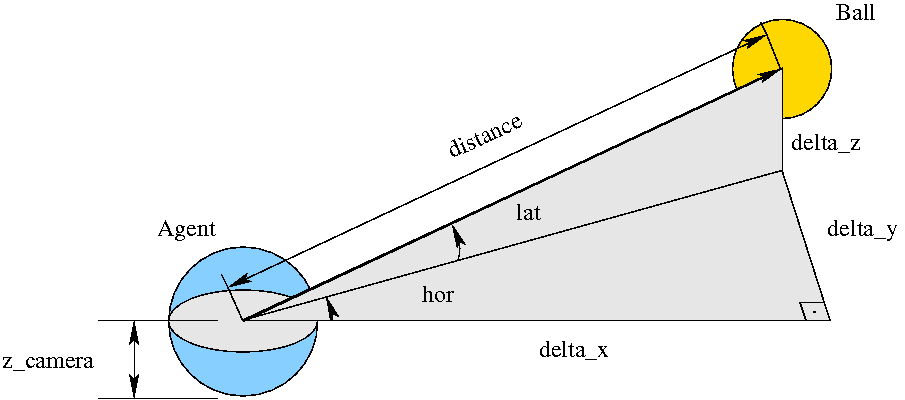
\includegraphics[scale=0.4]{fig/polar_conversion}
  \includegraphics[scale=1.4]{fig/agent_vision}
  \caption{Polar coordinates as supplied by the 3D Soccer Server}
  \label{fig:polarcoordinates}
\end{figure}

Contrary to 2D soccer simulation, the vision system does not deliver
object velocities. Objects can be occluded by other objects (this is
not completely implemented yet). All distances and angles are given
relative to the position and orientation of the camera.

% Klaus: where is it in humanoid league
% Joschka: in the head for most of them, although some robots have an additional camera on the torso pointing down to be able to see the ball if it's right in front of their feet.

The noise parameters of the vision system are as follows:
\begin{itemize}
  \item A small calibration error is added to the camera position. For each
  axis, the error is uniformly distributed between $-0.005 m$ and $0.005 m$. The
  error is calculated once and remains constant during the complete match.
  \item Dynamic noise normally distributed around $0.0$:
      \subitem - distance error: $\sigma = 0.0965$ (also, distance error is
      multiplied by $distance/100$)
      \subitem - horizontal angle error: $\sigma = 0.1225$
      \subitem - latitudal angle error: $\sigma = 0.1480$
\end{itemize}

A vision message is started with ``\texttt{See}'' followed by a list of seen
objects. While the ball and the markers on the field are simple objects described
through just one position vector, a player is a more complex object and needs a
tighter description as well as additional information like teamname or
player number. Therefore a player is described through the name of it's team,
the player number and one or more position vectors to different body parts.
According to the hyper complex image processing software attached to the vision
system :) the visual information are just percepted every third cycle.

In older server versions players are also described with just one position
vector. In this case the message format to the player differs as shown by the
simple player message format below.
\begin{itemize}
	\item[Message format:] \texttt{(See +(<name> (pol <distance> <angle1>
	<angle2>)) +(P (team <teamname>)\newline (id <playerID>) +(<bodypart>
	(pol <distance> <angle1> <angle2>))))}
	\item[Simple player format:] \texttt{(P (team <teamname>) (id <playerID>)
	(pol <distance> <angle1> <angle2>))}
		\begin{itemize}
		  \item[\texttt{<name>} -] the name of the visible object (see table
		  \ref{table:visible_objects} for possible values)
		  \item[\texttt{<distance>} -] the distance to the visible object in meters
		  and an accuracy of two digits
		  \item[\texttt{<angle1> <angle2>} -] the horizontal and latitudal angles to
		  the visible object in degrees and an accuracy of two digits
		  \item[\texttt{<teamname>} -] the name of the team, to which the seen player
		  belongs
		  \item[\texttt{<playerID>} -] the player number of the seen player
		  \item[\texttt{<bodypart>} -] the name of the body part (see table
		  \ref{table:visible_bodyparts} for possible values)
		\end{itemize}
	\item[Example message:] \texttt{(See 
    (G2R (pol 17.55 -3.33 4.31)) 
    (G1R (pol 17.52 3.27 4.07)) 
    (F1R (pol 18.52 18.94 1.54)) 
    (F2R (pol 18.52 -18.91 1.52)) 
    (B (pol 8.51 -0.21 -0.17)) 
    (P (team teamRed) (id 1) 
        (head (pol 16.98 -0.21 3.19)) 
        (rlowerarm (pol 16.83 -0.06 2.80)) 
        (llowerarm (pol 16.86 -0.36 3.10)) 
        (rfoot (pol 17.00 0.29 1.68)) 
        (lfoot (pol 16.95 -0.51 1.32))) 
    (P (team teamBlue) (id 3) 
        (rlowerarm (pol 0.18 -33.55 -20.16)) 
        (llowerarm (pol 0.18 34.29 -19.80))))}
	\item[Noise model:] Calibration error and dynamic noise
\end{itemize}



\begin{table}
\centering
\begin{tabular}[htbp]{|l|l|}
  \hline
  {\bf Simple visible object} & {\bf Identifier} \\
  \hline\hline
  Ball & \texttt{B}\\ \hline
  Flags & \texttt{F1L}, \texttt{F2L}, \texttt{F1R}, \texttt{F2R} \\ \hline
  Goalposts & \texttt{G1L}, \texttt{G2L}, \texttt{G1R}, \texttt{G2R} \\
  \hline
\end{tabular}
\caption{Simple visible objects.}
\label{table:visible_objects}
\end{table}%

\begin{table}
\centering
\begin{tabular}[htbp]{|l|l|}
  \hline
  {\bf Visible body part} & {\bf Identifier} \\
  \hline\hline
  Head & \texttt{head} \\ \hline
  Right lower arm & \texttt{rlowerarm} \\ \hline
  Left lower arm & \texttt{llowerarm} \\ \hline
  Right foot & \texttt{rfoot} \\ \hline
  Left foot & \texttt{lfoot} \\
  \hline
\end{tabular}
\caption{Visible body parts of the Nao robot.}
\label{table:visible_bodyparts}
\end{table}%


% What about the Restricted Vision Perceptor?
% The current soccer bot seems not to use it, still experimental/unsupported?

% Joschka: I'm not sure either. Oliver worked on that, and Yuan had several patches for it last year. Maybe Yuan has the best overview right now? The current Soccerbot doesn't use it.
% Hedayat: Currently Nao robot uses this perceptor.



%-SUB-SUB-SECTION---------------------------------------------------
%---------------------- AgentState Perceptor -----------------------
%-------------------------------------------------------------------
\subsubsection{AgentState Perceptor}
\label{sec:agentstateperceptor}
The \emph{agent state perceptor} gives information about the internal state of
the agent. It reports information about the current battery status and
the temperature of the agent.

\begin{itemize}
	\item[Message format:] \texttt{(AgentState (temp <degree>) (battery <percentile>))}
	\item[Example message:] \texttt{(AgentState (temp 48) (battery 75))}
\end{itemize}



%-SUB-SUB-SECTION---------------------------------------------------
%----------------------- GameState Perceptor -----------------------
%-------------------------------------------------------------------
\subsubsection{GameState Perceptor}
\label{sec:gamestateperceptor}
The \emph{game state perceptor} delivers several information about the actual
state of the soccer game environment. A game state message is started with the
``\texttt{GS}'' identifier, followed by a list of different state information.
Currently just the actual play time and play mode are transmitted, while the
play time starts from zero at kickoff of either half and is given as a floating
number in seconds. The possible play modes are listed in table
\ref{table:playmodes}. For an up to date list of all play modes refer to
(./plugin/soccer/soccertypes.h).

\begin{itemize}
	\item[Message format:] \texttt{(GS (t <time>) (pm <playmode>))}
	  \begin{itemize}
	    \item[\texttt{<time>} -] the current play time in seconds and two digits
	    \item[\texttt{<playmode>} -] the current play mode of the soccer game (see
	    table \ref{table:playmodes} for possible values)
	  \end{itemize}
	\item[Example message:] \texttt{(GS (t 0.00) (pm BeforeKickOff))}
\end{itemize}

\begin{table}
\centering
\begin{tabular}[htbp]{|l|l|}
  \hline
  {\bf Play mode} & {\bf Description} \\
  \hline\hline
  \texttt{BeforeKickOff} & before the match \\ \hline
  \texttt{KickOff\_Left} & kick off for the left team \\ \hline
  \texttt{KickOff\_Right} & kick off for the right team \\ \hline
  \texttt{PlayOn} & regular game play \\ \hline
  \texttt{KickIn\_Left} & kick in left team \\ \hline
  \texttt{KickIn\_Right} & kick in right team \\ \hline
  \texttt{CORNER\_KICK\_LEFT} & corner kick left team \\ \hline
  \texttt{CORNER\_KICK\_RIGHT} & corner kick right team \\ \hline
  \texttt{GOAL\_KICK\_LEFT} & goal kick for left team \\ \hline
  \texttt{GOAL\_KICK\_RIGHT} & goal kick for right team \\ \hline
  \texttt{OFFSIDE\_LEFT} & offside for left team \\ \hline
  \texttt{OFFSIDE\_RIGHT} & offside for right team \\ \hline
  \texttt{GameOver} & after the match \\ \hline
  \texttt{Goal\_Left} & goal scored by the left team \\ \hline
  \texttt{Goal\_Right} & goal scored by the right team \\ \hline
  \texttt{FREE\_KICK\_LEFT} & free kick for left team \\ \hline
  \texttt{FREE\_KICK\_RIGHT} & free kick for right team \\ \hline
  \texttt{NONE} & no or unknown play mode\\
  \hline
\end{tabular}
\caption{Possible play modes.}
\label{table:playmodes}
\end{table}%



%-SUB-SUB-SECTION---------------------------------------------------
%------------------------- Hear Perceptor --------------------------
%-------------------------------------------------------------------
\subsubsection{Hear Perceptor}
\label{sec:hearperceptor}
Agent processes are not allowed to communicate with each other directly, but
agents may exchange messages via the simulation server. For this purpose
agents are equipped with the so-called \emph{hear perceptor}, which serves as
an aural sensor and receives messages shouted by other players. Actually the
underlying model stems from the 2D Soccer Simulation and has been integrated 
in the 3D~simulator since server version~0.4. Percepts have the following format:
\begin{itemize}
	\item[Message format:] \texttt{(hear <time>	'self'|<direction> <message>)}
		\begin{itemize}
	  	  \item[\texttt{<time>} -] the play time when the given message was heard
	  	  in seconds
	  	  \item[\texttt{<direction>} -] the horizontal direction where the sound was
	  	  located, relative to the head in degrees
		  \item[\texttt{<message>} -] up to 20 characters, which may be taken
		  from the ASCII  printing character subset $[{\tt 0x20}, {\tt 0x7E]}$ except
		  the {\it white space}  character ($\sqcup$) and the {\it normal brackets}
		  {\tt(} and {\tt )}
		\end{itemize}
	\item[Example message:]	\texttt{(hear 12.30 self helloworld)}
\end{itemize}
The source is either the relative direction in degrees where the sound was
located, or {\tt self} if the player has a statement by his own. $Message$ may
consist of characters from the ASCII printing character subset \mbox{$[{\tt
0x20}, {\tt 0x7E]}$}, among which the alphanumerical symbols and mathematical
operators can be found for example. Three characters from this range are,
however, excluded: the {\it white space} character ($\sqcup$) and the normal
brackets {\tt(} and {\tt )}.

The hear perceptor comes up with some restrictions:
\begin{enumerate}
	\item Messages are restricted to a \emph{maximal length} (currently 20 bytes).
	\item Messages shouted from beyond a \emph{maximal distance} (currently $50.0$ meters) cannot be heard.
	\item The \emph{number of messages} which can be heard at the same time is
	bounded: Each player has the maximal capacity of one heard message by a
	specific team every two sensor cycles (thus every $0.4$ seconds per team).
	There are separately tracked capacities for both teams, because teams should
	not be able to block the hear perceptors of their opponents by shouting
	permanently. If more messages from players of one team arrive, they are
	processed in the order of arrival; the remaining messages are simply not
	heard.\\ Messages shouted by oneself, though, can always be noticed
	\cite{Vorst06}.
\end{enumerate}





%-SECTION-----------------------------------------------------------
%----------------------- Effectors/Actuators -----------------------
%-------------------------------------------------------------------
\section{Effectors/Actuators}
\label{sec:effectors}

Effectors are used to act within the simulation. They are sent to the server
to change the game state accordingly. There are effectors that are available to
all kinds of simulations and soccer specific effectors.

%Klaus: do we have noise in effectors?
% Joschka: only in the old kick effector (we need noise models though, should be a ToDo)

%Klaus: What are the minimal/maximal values to pass? What happens in case of errors
% Joschka: Good question ;-) For the joint effectors, you supply angles in degrees, there should be no problem. For anything else, I'm not sure.





%-SUB-SECTION-------------------------------------------------------
%------------------------ General Effectors ------------------------
%-------------------------------------------------------------------
\subsection{General Effectors}
\label{sec:generaleffectors}
The effectors described in this subsection are available to all types of
simulation. In other words they are not specific to the soccer environment.



%-SUB-SUB-SECTION---------------------------------------------------
%------------------------- Create Effector -------------------------
%-------------------------------------------------------------------
\subsubsection{Create Effector}
\label{sec:createeffector}
When an agent initially connects to the server it is invisible and
cannot take affect a simulation in any meaningful way. It only
possesses a so called \emph{create effector}.

An agent uses this effector to advice the server to construct it
according to a scene description file it passes as a parameter. This
file is used to construct the physical representation and all further
effectors and preceptors.

\begin{itemize}
	\item[Message format:] \texttt{(scene  <filename>)}
	\item[Example message:] \texttt{(scene rsg/agent/nao/nao.rsg)}
\end{itemize}

After the agent representation is constructed in the server the agent
should do further simulation specific setup. For example in the soccer
simulation each agent is required to register to a team and acquire a
unique player number. For these tasks usually a special effector like
the SoccerInitEffector is used.



%-SUB-SUB-SECTION---------------------------------------------------
%----------------------- HingeJoint Effector -----------------------
%-------------------------------------------------------------------
\subsubsection{HingeJoint Effector}
\label{sec:HJE}
A \emph{hinge joint effector} represents an actuator, related to a single axis
hinge joint. It is able to move the joint along the specific axis of freedom.
The first parameter is the name of the hinge joint effector (see robot
descriptions \ref{cha:robots}). The second parameter specifies the angular
change rate of the given hinge joint in degrees per cycle ($deg/cycle$). If the
requested angle change needs more force than the maximum allowed force for the
joint, then the maximum force will be used instead.

\begin{itemize}
	\item[Message format:] \texttt{(<name> <ax>)}
		\begin{itemize}
		  \item[\texttt{<name>} -] the name of the corresponding hinge joint
		  \item[\texttt{<ax>} -] the angular change rate in $deg/cycle$ (max joint
		  speed $7.035 deg/cycle$)
		\end{itemize}
	\item[Example message:] \texttt{(lae3 5.3)}
\end{itemize}



%-SUB-SUB-SECTION---------------------------------------------------
%--------------------- UniversalJoint Effector ---------------------
%-------------------------------------------------------------------
\subsubsection{UniversalJoint Effector}
\label{sec:UJE}
A \emph{universal joint effector} represents an actuator, related to a two axes
universal joint. It is able to move the joint along the two specific axis of
freedom. It starts with the name of the universal joint effector (see robot
descriptions \ref{cha:robots}), followed by the two angular velocities in
degrees per cycle. If the requested angle change needs more force than the
maximum allowed force for the joint, then the maximum force will be used
instead.

\begin{itemize}
	\item[Message format:] \texttt{(<name> <ax1> <ax2>)}
		\begin{itemize}
		  \item[\texttt{<name>} -] the name of the corresponding universal joint
		  \item[\texttt{<ax1> <ax2>} -] the angular change rates in $deg/cycle$ (max joint
		  speed $7.035 deg/cycle$) 
		\end{itemize}
	\item[Example message:] \texttt{(lae1\_2 -2.3 1.2)}
\end{itemize}





%-SUB-SECTION-------------------------------------------------------
%------------------------ Soccer Effectors -------------------------
%-------------------------------------------------------------------
\subsection{Soccer Effectors}
\label{sec:soccereffectors}
The following effectors are soccer specific and only available in the soccer
simulation.



%-SUB-SUB-SECTION---------------------------------------------------
%-------------------------- Init Effector --------------------------
%-------------------------------------------------------------------
\subsubsection{Init Effector}
\label{sec:initeffector}
The init command is sent once for each agent after the create effector sent the
scene command. It registers this agent as a member of the passed team with the passed number.
All players of one team have to use the same teamname and different numbers.
If an agent sends 0 as playernumber, the number is assigned automatically by
the server to the next free number.
The side on which a team starts to play depends on which team connected first.
\begin{itemize}
	\item[Message format:] \texttt{(init (unum <playernumber>)(teamname
	<yourteamname>))}
		\begin{itemize}
		  \item[\texttt{<playernumber>} -] the player number of the player
		  \item[\texttt{<yourteamname>} -] the name of the player's team
		\end{itemize}
	\item[Example message:] \texttt{(init (unum 1)(teamname FHO))}
\end{itemize}



%-SUB-SUB-SECTION---------------------------------------------------
%-------------------------- Beam Effector --------------------------
%-------------------------------------------------------------------
\subsubsection{Beam Effector}
\label{sec:beameffector}
The \emph{beam effector} allows a player to position itself on the field before
the game starts and after a goal was scored. The x and y coordinates define the
position on the field with respect to the coordinate system of figure
\ref{fig:pitch}. The rot value allows to define the horizontal direction of the
player. Zero degrees points to positive x axis, 90 degrees to positive y axis.
For reasons of simplification the position and rotation of the team playing from
right to left is point reflected on the field center.
\begin{itemize}
	\item[Message format:] \texttt{(beam <x> <y> <rot>)}
		\begin{itemize}
		  \item[\texttt{<x> <y>} -] target position on the soccer field in meter
		  \item[\texttt{<rot>} -] Z-rotation angle on target position in degrees
		\end{itemize}
	\item[Example message:] \texttt{(beam 10.0 -10.0 0.0)}
\end{itemize}



%-SUB-SUB-SECTION---------------------------------------------------
%-------------------------- Say Effector ---------------------------
%-------------------------------------------------------------------
\subsubsection{Say Effector}
\label{sec:sayeffector}

%klaus: is this old version only?
%Joschka: no, the Soccerbot has a say effector in the current version. It is restricted to 20 bytes msgs.
%description in TEXT_INSTEAD_... and Philipp Vorst's thesis
The \emph{say effector} permits communication among agents by broadcasting
messages. In order to say something, the following command has to be employed:
\begin{itemize}
	\item[Message format:] \texttt{(say <message>)}
		\begin{itemize}
		  \item[\texttt{<message>} -] up to 20 characters, which may be taken
		  from the ASCII  printing character subset $[{\tt 0x20}, {\tt 0x7E]}$ except
		  the {\it white space}  character ($\sqcup$) and the {\it normal brackets}
		  {\tt(} and {\tt )}
		\end{itemize}
	\item[Example message:] \texttt{(say helloworld)}
\end{itemize}
For further details and restrictions please see Section~\ref{sec:hearperceptor},
about the \emph{hear perceptor}, the dual sensor to this actuator.





%-SUB-SECTION-------------------------------------------------------
%--------------------- Older Version Effectors ---------------------
%-------------------------------------------------------------------
\subsection{Older Version Effectors}
\label{sec:olderversioneffectors}
The effectors in this subsection have been available in older versions of the
simulation and are now no longer available



%-SUB-SUB-SECTION---------------------------------------------------
%-------------------------- Drive Effector -------------------------
%-------------------------------------------------------------------
\subsubsection{Drive Effector}
\label{sec:driveeffector}
To use the omnidrive of the agent, you have to use the so called
"DriveEffector", which takes a cartesian vector (x y z) with a maximum
length of 100 units. The x-coordinate points towards the opponents
team side of the field, z points up. With the DriveEffector, you set a
kind of motor force, i.e. if you want to drive full speed for a while,
it is sufficient to use the DriveEffector *once*. The force you set is
applied at each simulator step until you change it again. The
DriveEffector works reliable, there is a small error for forces along
each axis (each up to 2\% of the applied force). The error is normally
distributed around $0.0$.

Using the omnidrive consumes battery. You get to know of battery
states by reading the AgentStatePerceptor. If the battery is empty,
the omnidrive will stop working. It is also possible to push away
other robots. Using this feature to push away opponents is discouraged
:).

\begin{itemize}
	\item[Message format:] \texttt{(drive <x> <y> <z>)}
	\item[Example message:] \texttt{(drive 20.0 50.0 0.0)}
\end{itemize}



%-SUB-SUB-SECTION---------------------------------------------------
%-------------------------- Kick Effector --------------------------
%-------------------------------------------------------------------
\subsubsection{Kick Effector}
\label{sec:kickeffector}
To move the ball, you have the option of simply using the robots to
push the ball into a desired direction, or you can use the
kickeffector to kick the ball. Originally, we did not intend to create
an artificial kickeffector. However, to make use of the 3rd dimension,
this was the easiest way. It is intended to remove this kind of kick
effector in future versions (not this years' competition) in favor of
a real physical device.

The kickeffector can accelerate the ball radially away from the robot
body. The kickeffector takes an angle as first argument. This is the
latitudal angle (in degrees) for accelerating the ball. It is
restricted to a number between 0 and 50. The second argument indicates
the kicking power and this is a number between 0 and 100. It is
interpreted as the percentile of the maximum available power. The
kickeffector adds a force and a torque to the ball. This happens over
a fixed number of simulation steps. Currently 10 cycles are used. This
corresponds to $1/10s$ simulation time. To kick the ball, the ball has
to be very close to the robot, i.e. it has to be within the so called
kickable margin of the player. Currently $0.04m$ are configured.

You cannot change the kicking angle in the horizontal plane. This
means that you have to move the robot so that it can kick into the
desired direction. Right now, the kickeffector is not very strong,
because something like an offside rule is missing. It should also not
be possible to move other robots by kicking the ball against them
anymore. (at least not very much :) Like the DriveEffector, the
kickeffector does only work if the robot touches the soccer field.

The kickeffector noise has the following parameters: 
\begin{itemize}
\item The angle error in the x-y plane is quite low and normally distributed
around $0.0$ with $\sigma = 0.02$.
\item The latitudal angle error is normally distributed around $0.0$. This
angle error is low with $\sigma = 0.9$ at both extreme positions, i.e. 0
and at 50 degrees. Towards the middle of the range the angle error
gets higher with sigma up to 4.5.
\item The kick power error is normally distributed around $0.0$ with $\sigma =
0.4$
\end{itemize}

\begin{itemize}
	\item[Message format:] \texttt{(kick <angle> <power>)}
	\item[Example message:] \texttt{(kick 20.0 80.0)}
\end{itemize}

% illustration from Philipp's thesis here?



%-SUB-SUB-SECTION---------------------------------------------------
%-------------------------- Catch Effector -------------------------
%-------------------------------------------------------------------
\subsubsection{Catch Effector}
\label{sec:catcheffector}
The goalie (agent number 1) is the only player with the ability to
catch a ball. The goalie can catch the ball in play mode 'playe\_on',
if the ball is inside the penalty area and close to the robot, i.e. it
has to be within the so called catch margin of the player. The current
value of catch margin is 2 meters.

The catcheffector puts the ball in front of the goalie on the ground
and moves players away that are closer than 2 meters to the goalie by
5 meters.

\begin{itemize}
	\item[Message format:] \texttt{(catch)}
	\item[Example message:] \texttt{(catch)}
\end{itemize}

% illustration from Philipp's thesis here?





%-SECTION-----------------------------------------------------------
%---------------------- Simulation Update Loop ---------------------
%-------------------------------------------------------------------
\section{Simulation Update Loop}
SimSpark implements a simple internal event model that immediately
executes every action received from an agent. It does not try to
compensate any network latency or compensate for different computing
resources available to the connected agents.

A consequence is that SimSpark currently does not guarantee that
events are reproducible. This means repeated simulations may have a
different outcome, depending on network delays or load variations on
the machines hosting the agents and the server.

A benefit of the simple structure however are speed gains that make it
interesting for machine learning tasks as in these setups an often
large number of different agent and simulation configurations are
repeatedly tested.

Further the SimSpark main loop is highly customizable as it is
entirely build upon plugins we call simcontrol nodes. Simcontrol nodes
are registered to the simulation server. They act in response to
control events. The simulation server repeatedly generates these as it
executes an abstracted the main loop.

The event types are an 'init' event once when the simulation server
starts and a 'done' event on shutdown. The main then loop cycles
repeatedly through the 'start cycle', 'sense agent', 'act agent' and
'end cycle' events.

Apart from generating control events the simulation server advances
the simulation time passed in the last cycle. Depending on its
configuration it either does this in discrete time quanta or in one
single step.

A simcontrol node further can take responsibility for the time
measurement, for example to synchronize the simulation time with the
real time used to render the scene.  Otherwise the simulation is
stepped a fixed time step as often as possible.

In this way all management tasks are implemented as plugins to the
simulation server. This involves the agent management, monitor
management, rendering, mouse and keyboard input and network code.

This setup allows us to configure the simulation at runtime as either
a monolithic application that does both simulation and rendering or as
a dedicated simulation server that defers rendering to a remote
monitor application.





%-SUB-SECTION-------------------------------------------------------
%---------------------- Single-threaded Timer ----------------------
%-------------------------------------------------------------------
\subsection{Single-threaded Timer}
In the singled-threaded mode, the main loop cycles repeatedly through
the `start cycle', `sense agent', `act agent' and `end cycle' events(
see \autoref{fig:single-thread-sd}). There are two noticeable details:
\begin{itemize}
\item Each cycle duration is $20ms$, if the simulation is fast than real
  time, it will wait; otherwise, if the simulation is very slow, it
  will run many physics updates once without interaction with agents.
  If the simulation is very slow, it will give up to catch up the real
  time and print warning. So you may have problem while the computer
  is not fast enough.
\item The `act agent' event is followed after `sense agent', the
  action which the agent send according to $n^{th}$ cycle will be
  realized in the $(n+1)^{th}$ cycle, i.e. the action has been delayed
  one cycle. See for \autoref{fig:synchronization} explanation.
\end{itemize}

\begin{figure}[htp]
  \centering
  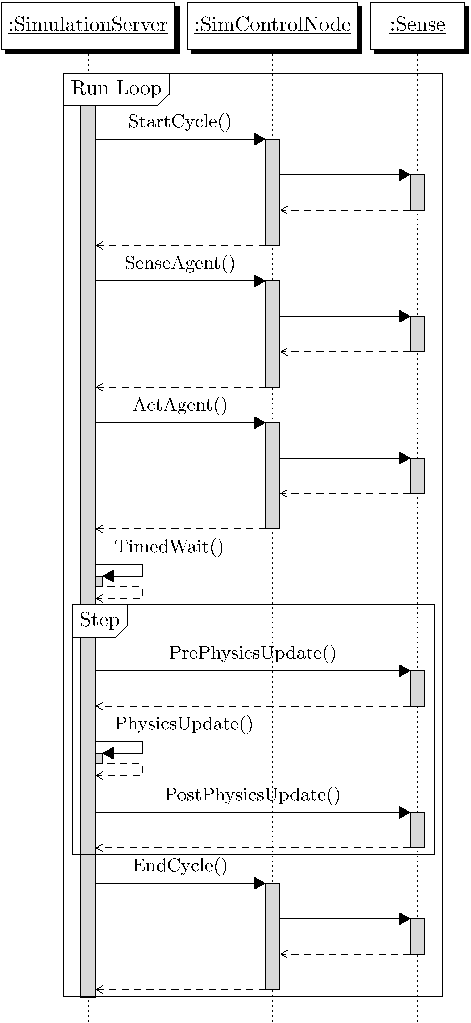
\includegraphics[height=0.6\textheight]{fig/serverSingleThreadLoop}
  \caption{Single-threaded loop UML sequence diagram}
  \label{fig:single-thread-sd}
\end{figure}

\begin{figure}[htp]
  \centering
  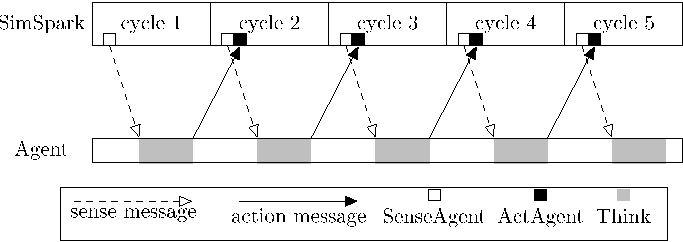
\includegraphics[width=0.8\textwidth]{fig/synchronization}
  \caption{Synchronization between SimSpark and agent}
  \label{fig:synchronization}
\end{figure}





%-SUB-SECTION-------------------------------------------------------
%----------------------- Multi-threaded Timer ----------------------
%-------------------------------------------------------------------
\subsection{Multi-threaded Timer}
In modern time, computers have more than one CPU or dual cores in one
CPU. This improve the performance greatly, but only the multi-threaded
program can benefit. SimSpark has an experimental multi-threaded
running loop, it can be switched on simply by change the
\texttt{simulationServer.setMultiThreads(false)} to
\texttt{simulationServer.setMultiThreads(true)} in the
\texttt{spark.rb} file.

The implementation of multi-threaded loop is based on two conditions.
First, every SimControlNode response for different parts of the
simulation, they perform one by one in the singled-threaded mode, but
they can run in parallel. Second, there is a active scene which stores
the whole simulation data in a tree. The physics engine and
SimControlNode interact through the active scene. As we know, the
physics computation is the most time-consuming, and the physics engine
does not need to access the active scene during physics computation.
So the physics computation and SimControlNodes can run in parallel. At
last, we get the multi-threaded simulation loop as
\autoref{fig:multi-thread-sd}. Note that the agent's action are also
delayed one cycle in the multi-threaded loop.
\begin{figure}[htp]
  \centering
  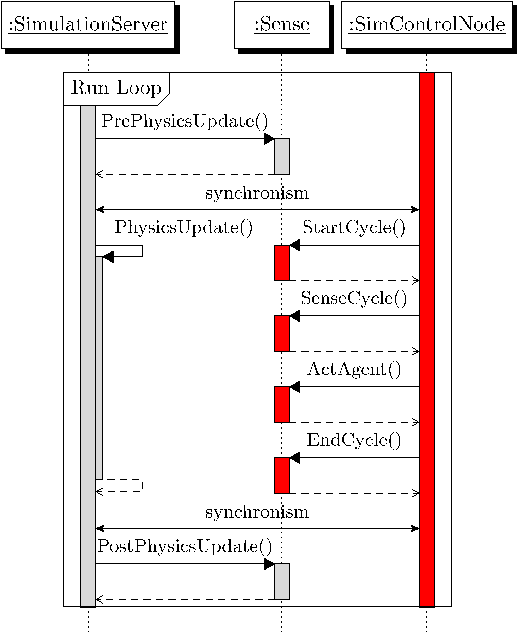
\includegraphics[height=0.5\textheight]{fig/serverMultiThreadLoop}
  \caption{Multi-threaded loop UML sequence diagram, note that
    each SimControlNode runs in separated thread.}
  \label{fig:multi-thread-sd}
\end{figure}

%----------------------------------------------------------------------
%\section{Setup Scripts}

%\textbf{TODO:}

%\begin{itemize}
%\item describe purpose of scripts in \~/.rcssserver3d/
%\item kerosin.rb for rendering configuration of simspark
%\end{itemize}

%%% Local Variables: 
%%% mode: latex
%%% TeX-master: "user-manual"
%%% End: 
